%!TEX root = zukaFinalReport.tex
%!TEX encoding = UTF-8 Unicode
%==============================================================================

%\section{Introduction}
Recently, robotics community witnesses excessive progress. In Spite of this progress, It still undergo complexity and significant challenges to the software developers; One of the main reasons for this issue is  handling the wide variation in tasks and environments of robot systems by an individual. 
ROS -Robot Operating System- is the flexible framework that makes robot software developing is more robust and accessible by robotics community. The official description of ROS is:
\begin{quotation}
``ROS is an open-source, meta-operating system for your robot. It provides the services you would expect from an operating system, including hardware abstraction, low-level device control, implementation of commonly-used functionality, message-passing between processes, and package management. It also provides tools and libraries for obtaining, building, writing, and running code across multiple computers.''
\end{quotation}
    
\section{Modularity}
The core of successive software algorithm is the ability to reuse in different projects without reimplementing. Modularity is an important Software principle. It divides complex systems into manageable and simpler modules 
ROS adds value to the most robotics projects and applications because of it Modularity, so you can use ROS as much as you desire and still implement your own parts.
\section{Distributed Nature }
Communication between multiple process  is the key to powerful system. ROS provides an integration point that able to manage hardware, drives, development tools, useful libraries, simulators and much more. 
A ROS distribution is a set of ROS software packages that can be downloaded
to your computer.


\section{Road Map to ROS development}
	\subsection{Filesystem Level}
The filesystem level explains how ROS files are organized on the hard disk.ROS program is divided into folders, and these Folders has some files that describe their functionality


\begin{description}
    \item[label] description
\end{description}
 		 \begin{description}
  			\item [Packages]
  				A package might contain ROS nodes, a ROS-independent library, a dataset, configuration files, a third-party piece of software, or anything else that logically constitutes a useful module.
  	\begin{figure}[ht]
  		\centering
  		\caption{Filesystem level representation}
  		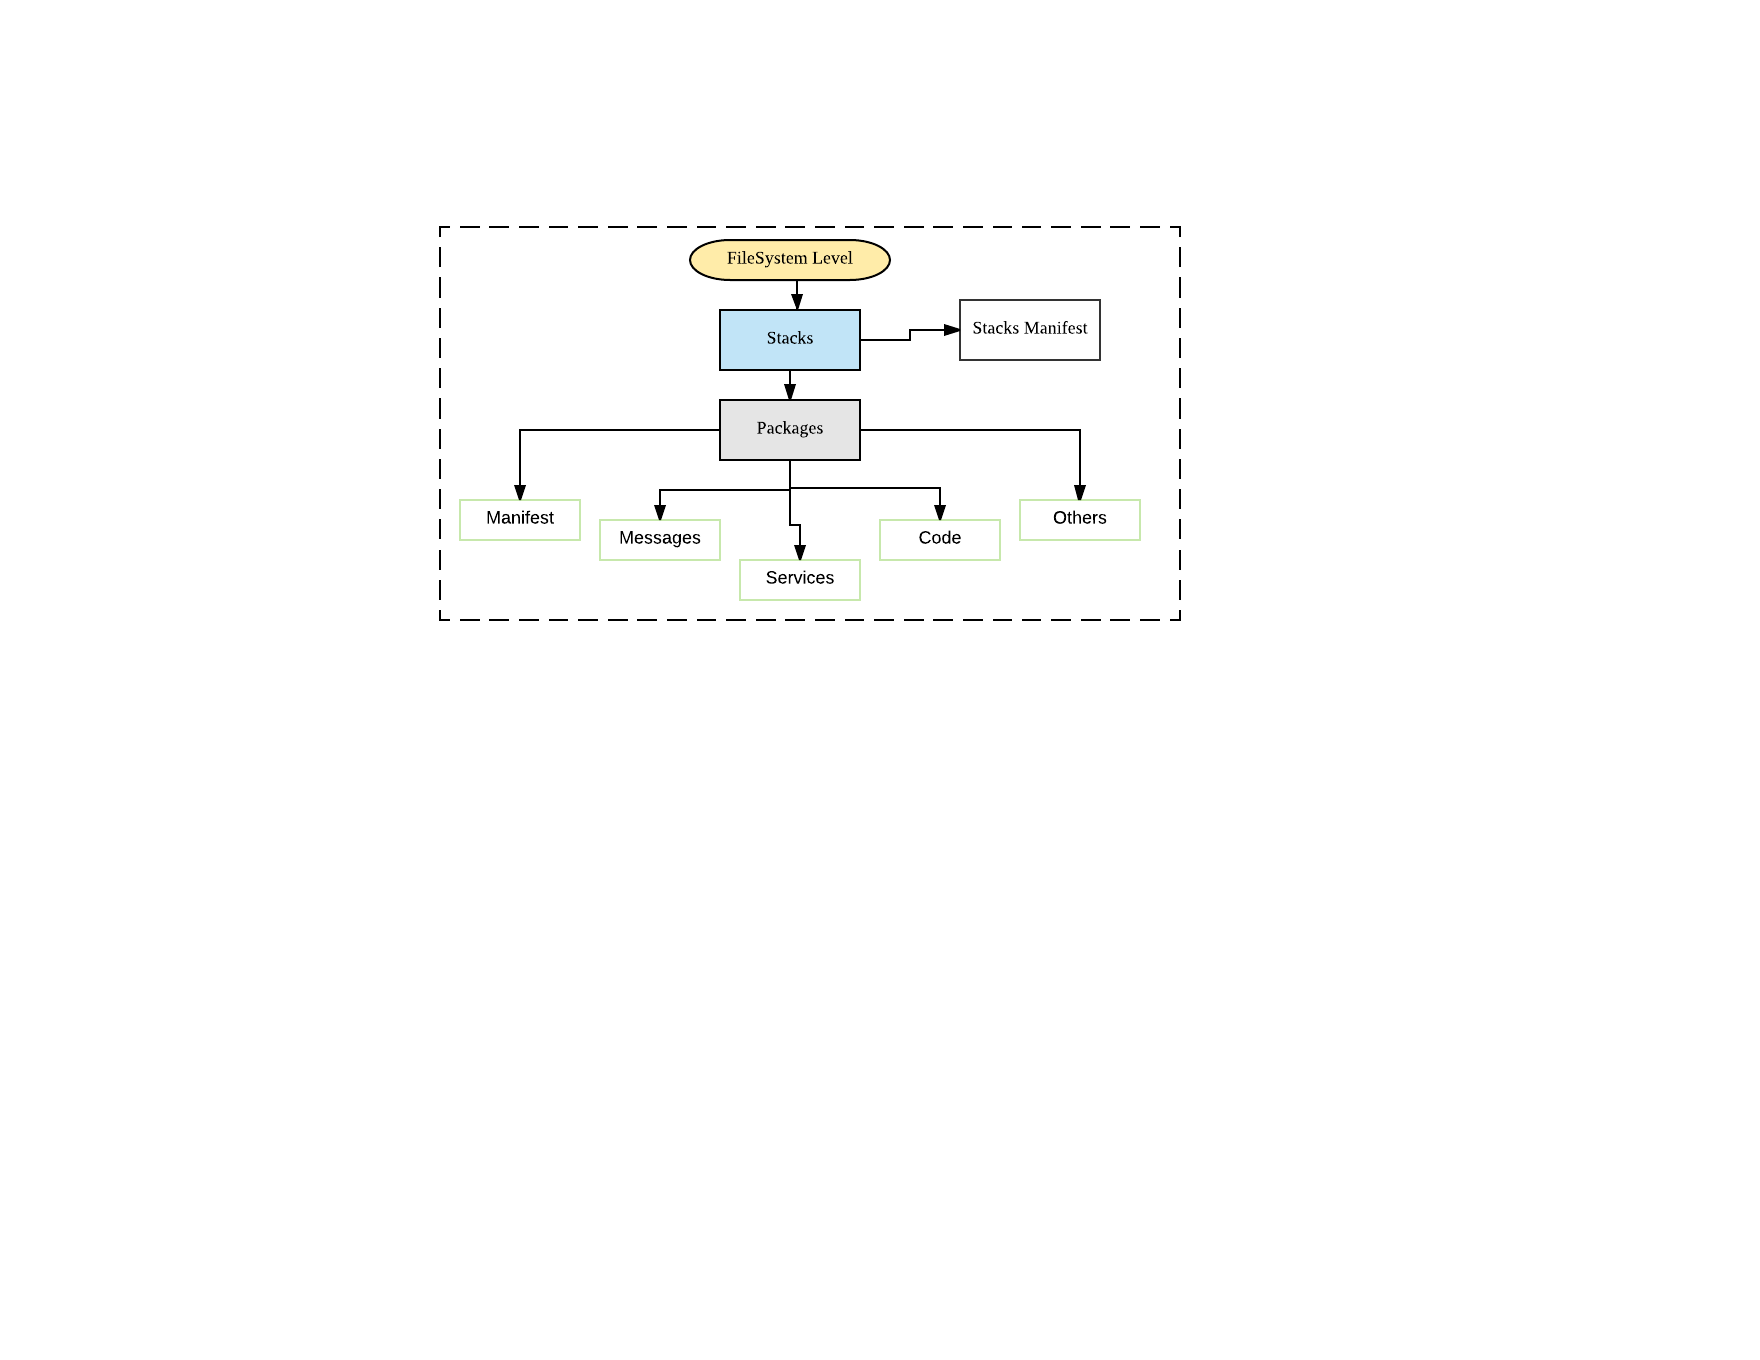
\includegraphics[scale=0.8]{BD1.jpeg}
  	\end{figure}
  			\paragraph{ROS Package tools }
  	To create, modify, or work with packages, ROS gives us some tools for assistance
  	\begin{table}[H]
  		\centering
  	\begin{tabular}{| p{3cm} |p{8cm}|}\hline
          Command  &  Function\\\hline\hline
          \texttt{rospack}  &  This command is used to get information or find packages in the system\\\hline
           \texttt{roscreate-pkg} & creating new package with your own dependencies \\\hline
           \texttt{rosmake} &  This command is used to compile package\\\hline
           \texttt{rosdep} &  This command installs system dependencies of a package\\\hline 
           \texttt{rxdeps} &  This command is used if you want to see the package dependencies as a graph\\\hline 
      \end{tabular}
  		\caption{ROS Package commands}
  		\label{table:1}
  	\end{table}
 \item [Stacks]
 Packages in ROS are organized into ROS stacks.the main goal of stacks is to ease the process of sharing codes.
 \item [Messages]
 Nodes communicate with each other by publishing messages to topics. A message is a simple data structure, comprising typed fields. Standard primitive types (integer, floating point, boolean, etc.)
 \item [Services]
 ROS uses simplified service description language for describing ROS service types. This builds directly upon the ROS msg format to enable request/response communication between nodes. Service descriptions are stored in .srv files. 
\end{description}

\subsection{Computaional Graph Level}
The basic Computation Graph concepts of ROS are: nodes, Master, Parameter Server, messages, services, topics, and bags, all of which provide data to the Graph in different ways.
\begin{itemize}
	\item Nodes: Nodes are processes where computation is done. A system better has many nodes to control different functions. Nodes are written with ROS client library; roscpp, or rospy.
	\item Master: ROS Master is the part that facilitates all the communication between nodes.You should allow the master to continue running for the entire time that you’re using ROS.
	\item Parameter Server: The Parameter Server gives us the possibility to have data stored using keys in a central location.
	\item  Messages: The Parameter Server gives us the possibility to have data stored using keys in a central location.
	\item Topics: Messages are organized into topics. Nodes that need to listen to certain messages will \textbf{subscribe} to the topics that it is interested in, or if the node wants to share it is information, the node will \textbf{publish}to an appropriate topic.
	\begin{figure}[H]
		\centering
		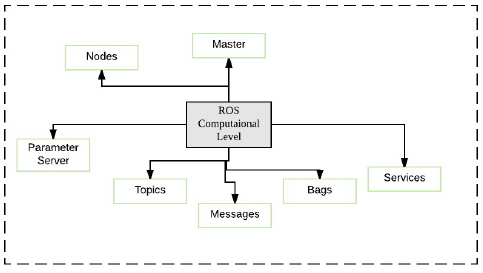
\includegraphics[scale=0.8]{bd2.jpg}
        		\caption{Filesystem level representation}
	\end{figure}
\end{itemize}

\subsection{Community Level}
The third level is the Community level where you can find useful resources and interact with different developers to exchange knowledge, algorithms, and softwares.
The official description of ROS Community level resources:

\textit{\begin{itemize}
\item  Distributions: ROS Distributions are collections of versioned stacks that you can install. Distributions play a similar role to Linux distributions: they make it easier to install a collection of software, and they also maintain consistent versions across a set of software.
\item Repositories: ROS relies on a federated network of code repositories, where different institutions can develop and release their own robot software components.
\item The ROS Wiki: The ROS community Wiki is the main forum for documenting information about ROS. Anyone can sign up for an account and contribute their own documentation, provide corrections or updates, write tutorials, and more.
\item Bug Ticket System: Please see Tickets for information about file tickets.
\item  Mailing Lists: The ros-users mailing list is the primary communication channel about new updates to ROS, as well as a forum to ask questions about ROS software.
\item  ROS Answers: A Q and A site for answering your ROS-related questions.
\item Blog: The Willow Garage Blog provides regular updates, including photos and videos.
\end{itemize}}
 
\paragraph{ROS tutorials}
\url{wiki.ros.org/ROS/Tutorials}

\section{Using Sensors with ROS: Kinect}
\begin{figure}[h]
    \centering
    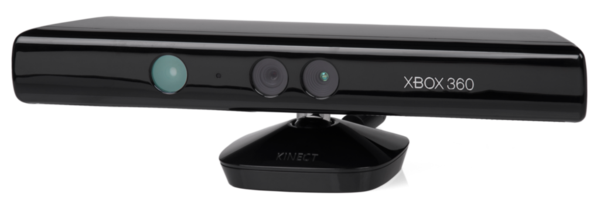
\includegraphics[width=0.7\textwidth]{kinect.png}
    \caption{Kinect Xbox 360 with RGB Camera, Depth Camera, and Microphone array}
\end{figure}
\subsection{Operation and Inferring body position}
%\paragraph{Inferring body position}
The process of inferring body position done by two main stages: analyzing a speckle pattern of infrared laser light to produce depth map; then transforms depth image to
body part image from motion capture system and finally transforms the body part
image into a skeleton.
\begin{figure}[h]
	\centering
	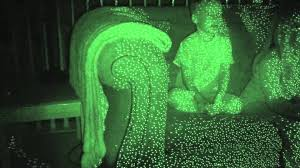
\includegraphics[scale=0.9]{IRLight_bykinect.jpeg}
    	\caption{Speckle Pattern}
\end{figure}
 
 \subsection{OpenNI: Natural Interaction}
 The term natural interaction refers to people communicating with devices through their human senses, such as audio, and vision. The most obvious applications uses this technology are: face/ voice recognition; body motion tracking; and control room electronics using hand gesture
 
 \paragraph{Abstract Layered View}
The three layered view of OpenNI :
\begin{itemize}
\item \textbf{Top}: Represents the software that implements natural interaction applications on top of OpenNI.
\item \textbf{Middle}: Represents OpenNI, providing communication interfaces that interact with both the sensors and the middleware components, that analyze the data from the sensor..
\item \textbf{Bottom}: Shows the hardware devices that capture the visual and audio elements of the scene.
\end{itemize}

\subsection {Skeleton Tracking: User segmentation}
Skeleton tracker generate  data of the users who exist in the scene; these data includes location of the skeletal joints, and ability to track skeleton position.

There are some consideration for accurate skeleton tracking:
\begin{itemize}
	\item User considered to be lost if the user is not visible in the scene within 10 seconds
	\item Users get ID “user 1,2,...”. However the ID is recycled.
	\item Ideal distance for tracking around 2.5 m
	\item User should not wear very loose clothing, for better result.
\end{itemize}
\paragraph{Calibration}
To start tracking body, the user should do calibration position “psi pose” as shown in figure.
	\begin{figure}[H]
    \centering
    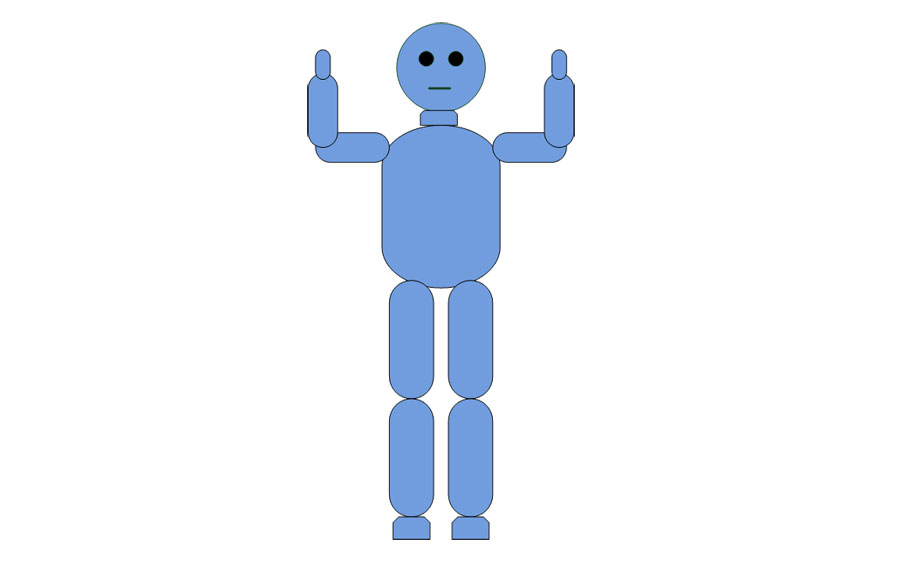
\includegraphics[width=0.90\textwidth]{calibrationpose2.jpg}
        \caption{PSI pose}
\end{figure}

      \paragraph {Limitations:}
\begin{itemize}
	\item User should not be sitting
	\item Most of the user body should be invisible
	\item User should be located 1 m away from kinect
\end{itemize}
\paragraph{Skeleton tracker output}
Skeleton tracker return the position, and quaternion of the joint.
%\begin{figure}
%\centering
%%\caption{Skeleton's Joint Coordinate representation}
%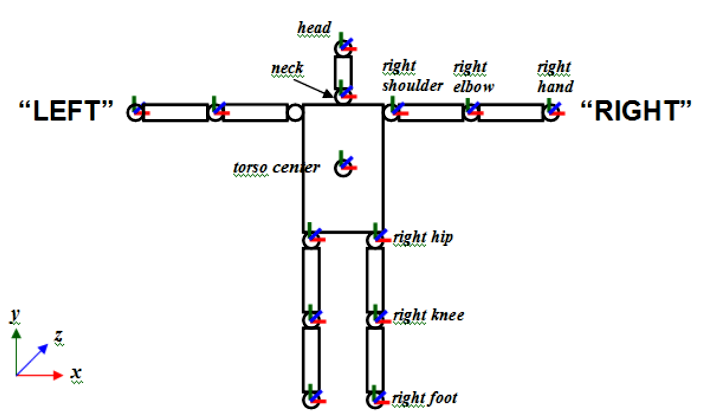
\includegraphics[scale=0.5]{coordinate_skeleton.png}
%\end{figure}

\paragraph{Joint Transformation}
Joint positions and orientations are given in the real world coordinate system. The origin of the system is at the sensor. The positive direction of X-axis is to the right of origin “, The positive direction of Y-axis is up, and The positive direction of Z-axis is in the direction of increasing depth. The coordinate frame is shown in the figure above.


Keep in mind that representation of the skeleton in Rviz supposed to be in Mirror mode which indicates that the LEFT side labeled in Rviz window is actually your RIGHT side.
\begin{figure}[ht]
	\centering
	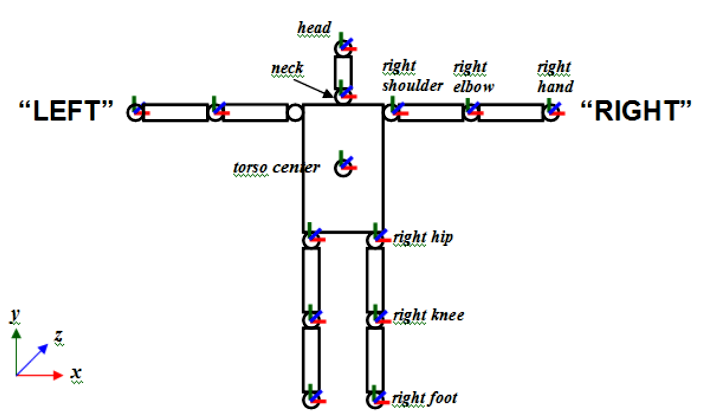
\includegraphics[width=0.8\textwidth]{coordinate_skeleton.jpg}
    	\caption{Skeleton joints Coordinate}
\end{figure}
Joint positions are measured in units of m and orientations are  in radians.

\subsection{Kinect Driver}
\paragraph{Openni launch Package} This package contains launch files for using OpenNI-compliant devices such as the Microsoft Kinect in ROS.  from the device driver into point clouds, disparity images, and other products suitable for processing and visualization.

to open Kinect device and transform raw data to convenient data, run this command:
\begin{lstlisting}[language=terCmd]
$ roslaunch openni_launch openni.lanuch
\end{lstlisting}


\paragraph{Openni tracker Package}
openni\_tracker broadcasts the OpenNI skeleton frames using tf.
this package allows you to track a person's skeleton using a Kinect. It also gives you the positions, relative to the camera frame
run this command:
\begin{lstlisting}[language=terCmd]
$ rosrun openni_tracker penni_tracker
\end{lstlisting}

Stand in front of the Kinect. If the terminal window where you ran openni\_tracker, you should see output like this:
\begin{lstlisting}[language=terCmd]
    [INFO]: New User 1
    [INFO]: Calibration started for user 1
    
    [INFO]: Calibration complete, start tracking user
\end{lstlisting}

\subsection{3D Visualizing}
As discussed in the previous sections, Kinect produced 3D data in form of point clouds.For this reason ROS has invented tool to visualize this type of data.
these tools enable you to develop robotic system faster by visualizing your data and evaluate the quality of result for validation.
\paragraph{Visualizing 3D data using rviz}
With roscore running, we only have to execute the following code to start rviz:
\begin{lstlisting}[language=terCmd]
$ rosrun rviz rviz
\end{lstlisting}

This command will open rviz interfac
% insert picture of Rviz interface
\begin{figure}[ht]
	\centering
	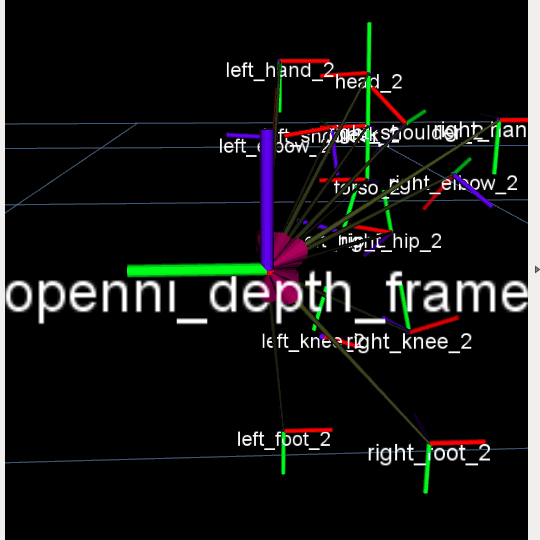
\includegraphics[scale=0.5]{rviz_tracker.jpg}
    	\caption{Visualizing skeleton joints using Rviz}
\end{figure}